\newcommand{\red}[1]{{\color{red}#1}}

\usetikzlibrary{shapes.multipart}

\tikzstyle{demoBox} = [
draw=blue!20, very thick,
rectangle split, rectangle split parts=2, rounded corners, inner xsep=0.5cm,
rectangle split part fill = {blue!20, blue!5}
]


\NewEnviron{nota}[1][]{%

\begin{center}
	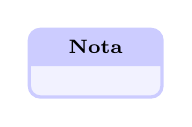
\begin{tikzpicture}
	\node [demoBox](box){%
		\textbf{\scriptsize 
			Nota}
		\nodepart{two}
		\begin{minipage}{0.8\textwidth}
		\vspace*{0.1cm}
		\BODY
		\end{minipage}
	};
	\end{tikzpicture}
\end{center}
}

\newcolumntype{L}[1]{>{\raggedright\arraybackslash\hsize=#1\hsize}X}
\newcolumntype{R}[1]{>{\raggedleft\arraybackslash\hsize=#1\hsize}X}
\newcolumntype{C}[1]{>{\centering\arraybackslash\hsize=#1\hsize}X}
